\section*{Спільна підготовка}

\markboth{Підготовка}{}

Дані Ames Housing містять 2930 продажів. SalePrice вимірюється в доларах
США, площі у квадратних футах. Рівень значущості 0.05, початкове
значення генератора 42. Розрахунки виконано в numpy, pandas, scipy,
statsmodels і scikit-learn; імпорти та оформлення графіків наведено лише
в notebook.

У множинних регресіях використовуємо 2414 повних спостережень.
MSSubClass і текстові ознаки кодуємо фіктивними змінними; базовий рівень
найчастіший. Не включаємо ідентифікатори Order та PID, GarageYrBlt (не
визначений без гаража), а також TotalBsmtSF і GrLivArea, які є точними
сумами інших площ. Категоріальні значення NA зберігаємо як окремі рівні.


\pythoncode{common}

\section{Задача 5: Лінійна регресія в Python}

\markboth{Задача 5}{}

\Needspace{329.0pt}

\subsection{(1) Тип житла та кодування категорій}

\begin{taskstatement}
Перед підгонкою моделі до даних спочатку детальніше розглянемо
визначення змінних та вирішимо, чи потребують деякі з них окремої
обробки. Розглянемо, наприклад, першу змінну MSSubClass. Вона набуває
текстових (категоріальних) значень і очевидно не може бути включена в
лінійну модель у вихідному вигляді. Існує два підходи до обробки такої
змінної. Один підхід полягає в присвоєнні чисел від 1 до 16 кожному
можливому результату (Label Encoding). Інший підхід полягає у створенні
нових фіктивних змінних (One-Hot Encoding / Dummy variables), які
дорівнюють одиниці для конкретного результату і нулю в іншому випадку.
Обговоріть ці два підходи та запропонуйте, який із них є більш доречним
у цьому випадку. Мотивуйте своє рішення, беручи до уваги номінальну,
порядкову та кардинальну шкали зі статистики. Запустіть просту регресію
SalePrice на MSSubClass у тому вигляді, в якому вона є (без кодування).
Перевірте, як statsmodels або scikit-learn обробляє такий тип змінної,
якщо вона передана як звичайний числовий тип (int64), та як її примусово
змінити на категоріальну за допомогою pd.Categorical або формул
statsmodels.formula.api.ols (C(MSSubClass)).
\end{taskstatement}


\pythoncode{p5-c5}

\Needspace{19.2pt}

\resulttext{p5-c5-out0.txt}

\begingroup\fontsize{7.5}{9.5}\selectfont\setlength{\tabcolsep}{2.5mm}\renewcommand{\arraystretch}{1.15}
\par\vspace{2pt}\noindent\begin{tabular}{|llll|}
\hline
 & Параметрів & R² & Скоригований R² \\
\hline
int64: один нахил & 2 & 0.00724058 & 0.00690152 \\
C(MSSubClass) & 16 & 0.247767 & 0.243895 \\
pd.Categorical & 16 & 0.247767 & 0.243895 \\
\hline
\end{tabular}\par\vspace{2pt}
\endgroup


\Needspace{37.599999999999994pt}

\resulttext{p5-c5-out2.txt}

\begingroup\fontsize{7.5}{9.5}\selectfont\setlength{\tabcolsep}{2.5mm}\renewcommand{\arraystretch}{1.15}
\par\vspace{2pt}\noindent\begin{tabular}{|lll|}
\hline
MSSub\allowbreak{}Class & count & mean \\
\hline
20 & 1079 & 187356 \\
30 & 139 & 96726.9 \\
40 & 6 & 144917 \\
45 & 18 & 111783 \\
50 & 287 & 137433 \\
60 & 575 & 239364 \\
70 & 128 & 156526 \\
75 & 23 & 199978 \\
80 & 118 & 168009 \\
85 & 48 & 149842 \\
90 & 109 & 139809 \\
120 & 192 & 208019 \\
150 & 1 & 148400 \\
160 & 129 & 137080 \\
180 & 17 & 107671 \\
190 & 61 & 125870 \\
\hline
\end{tabular}\par\vspace{2pt}
\endgroup


\begin{figure}[H]
\centering
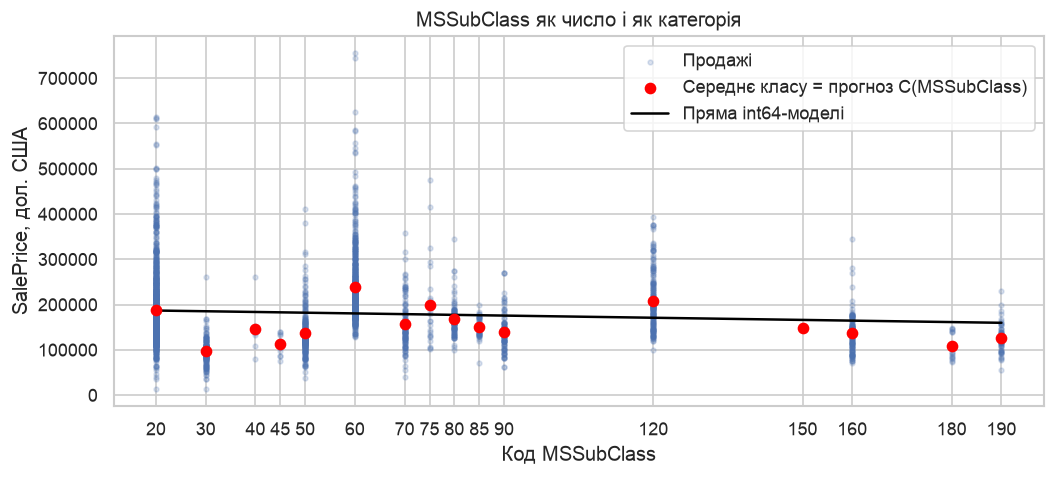
\includegraphics[width=\linewidth,height=0.82\textheight,keepaspectratio]{../../figures/problem5_mssubclass.png}
\caption{MSSubClass як числовий код і як категоріальна змінна.}
\end{figure}


\answerheading
\texttt{MSSubClass} записано числами (\texttt{int64}), але це коди типів
житла: код 20 означає одноповерховий будинок 1946 р. і новіший, код 30
такий самий будинок 1945 р. і старший, код 60 двоповерховий будинок, код
90 дуплекс. Це номінальна шкала:

\begin{itemize}
\item
  немає природного порядку (на відміну від порядкової шкали, наприклад
  оцінки якості 1--10);
\item
  різниця кодів не має змісту (на відміну від кардинальної, кількісної
  шкали, наприклад площі): \(60-20=40\) нічого не означає.
\end{itemize}

Label Encoding (номери 1--16 або самі коди) змусив би модель вважати, що
кожен крок коду змінює ціну на ту саму суму. One-Hot / фіктивні змінні
дають кожному класу власний зсув відносно базового класу. Тому тут
доречні фіктивні змінні. Для 16 класів беремо 15 індикаторів і
константу: усі 16 разом із константою дали б точну лінійну залежність
(пастка фіктивних змінних).

Що робить statsmodels:

\begin{itemize}
\item
  як \texttt{int64} змінна вважається звичайним числом, тому оцінюється
  один нахил: \(-159.43\) дол. на одиницю коду, \(R^2=0.0072\);
\item
  \texttt{C(MSSubClass)} у формулі або \texttt{pd.Categorical}
  перетворюють змінну на 15 фіктивних (базовий клас 20): 16 параметрів,
  \(R^2=0.2478\).
\end{itemize}

Обидва категоріальні способи дають однакові прогнози, а саме середню
ціну кожного класу (червоні точки на графіку). Наприклад, коефіцієнт
\texttt{C(MSSubClass){[}T.30{]}} \(=-90629\): клас 30 у середньому
дешевший за клас 20 на \(187356-96727\approx 90.6\) тис. дол. Чорна
пряма int64-моделі майже горизонтальна й не відображає цих різниць.


\Needspace{225.0pt}

\subsection{(2) Графічний аналіз}

\begin{taskstatement}
Розгляньте такі числові пояснювальні змінні: LotFrontage, LotArea,
YearBuilt, BsmtFinSF1, BsmtUnfSF. Побудуйте діаграму розсіювання
(scatter plot) залежності SalePrice від цих змінних за допомогою
matplotlib або seaborn. Проаналізуйте кожен графік та обговоріть
потенційні проблеми, трансформації або розширення моделі, які дозволять
врахувати виявлені закономірності. Пам'ятайте, що ви можете або
трансформувати наявні змінні (наприклад, np.log), або створювати нові
для фіксації нестандартних патернів.
\end{taskstatement}


\pythoncode{p5-c8}

\begingroup\fontsize{7.5}{9.5}\selectfont\setlength{\tabcolsep}{2.5mm}\renewcommand{\arraystretch}{1.15}
\par\vspace{2pt}\noindent\begin{tabular}{|lllll|}
\hline
 & count & min & 50\% & max \\
\hline
LotFrontage & 2440 & 21 & 68 & 313 \\
LotArea & 2930 & 1300 & 9436.5 & 215245 \\
YearBuilt & 2930 & 1872 & 1973 & 2010 \\
BsmtFinSF1 & 2929 & 0 & 370 & 5644 \\
BsmtUnfSF & 2929 & 0 & 466 & 2336 \\
\hline
\end{tabular}\par\vspace{2pt}
\endgroup


\Needspace{37.599999999999994pt}

\resulttext{p5-c8-out2.txt}

\begingroup\fontsize{7.5}{9.5}\selectfont\setlength{\tabcolsep}{2.5mm}\renewcommand{\arraystretch}{1.15}
\par\vspace{2pt}\noindent\begin{tabular}{|llll|}
\hline
Order & Значення & Sale\allowbreak{}Price & Змінна \\
\hline
1266 & 313 & 242000 & LotFrontage \\
1499 & 313 & 160000 & LotFrontage \\
957 & 215245 & 375000 & LotArea \\
1571 & 164660 & 228950 & LotArea \\
1499 & 5644 & 160000 & BsmtFinSF1 \\
2181 & 4010 & 183850 & BsmtFinSF1 \\
\hline
\end{tabular}\par\vspace{2pt}
\endgroup


\begingroup\fontsize{7.5}{9.5}\selectfont\setlength{\tabcolsep}{2.5mm}\renewcommand{\arraystretch}{1.15}
\par\vspace{2pt}\noindent\begin{tabular}{|llllll|}
\hline
Year\allowbreak{}Built & (1870, 1920] & (1920, 1950] & (1950, 1980] & (1980, 2000] & (2000, 2010] \\
\hline
count & 233 & 437 & 1050 & 475 & 735 \\
median & 119000 & 126000 & 142776 & 200000 & 226000 \\
std & 48793.2 & 49699.8 & 41030.8 & 73249.3 & 88353.9 \\
\hline
\end{tabular}\par\vspace{2pt}
\endgroup


\begin{figure}[H]
\centering
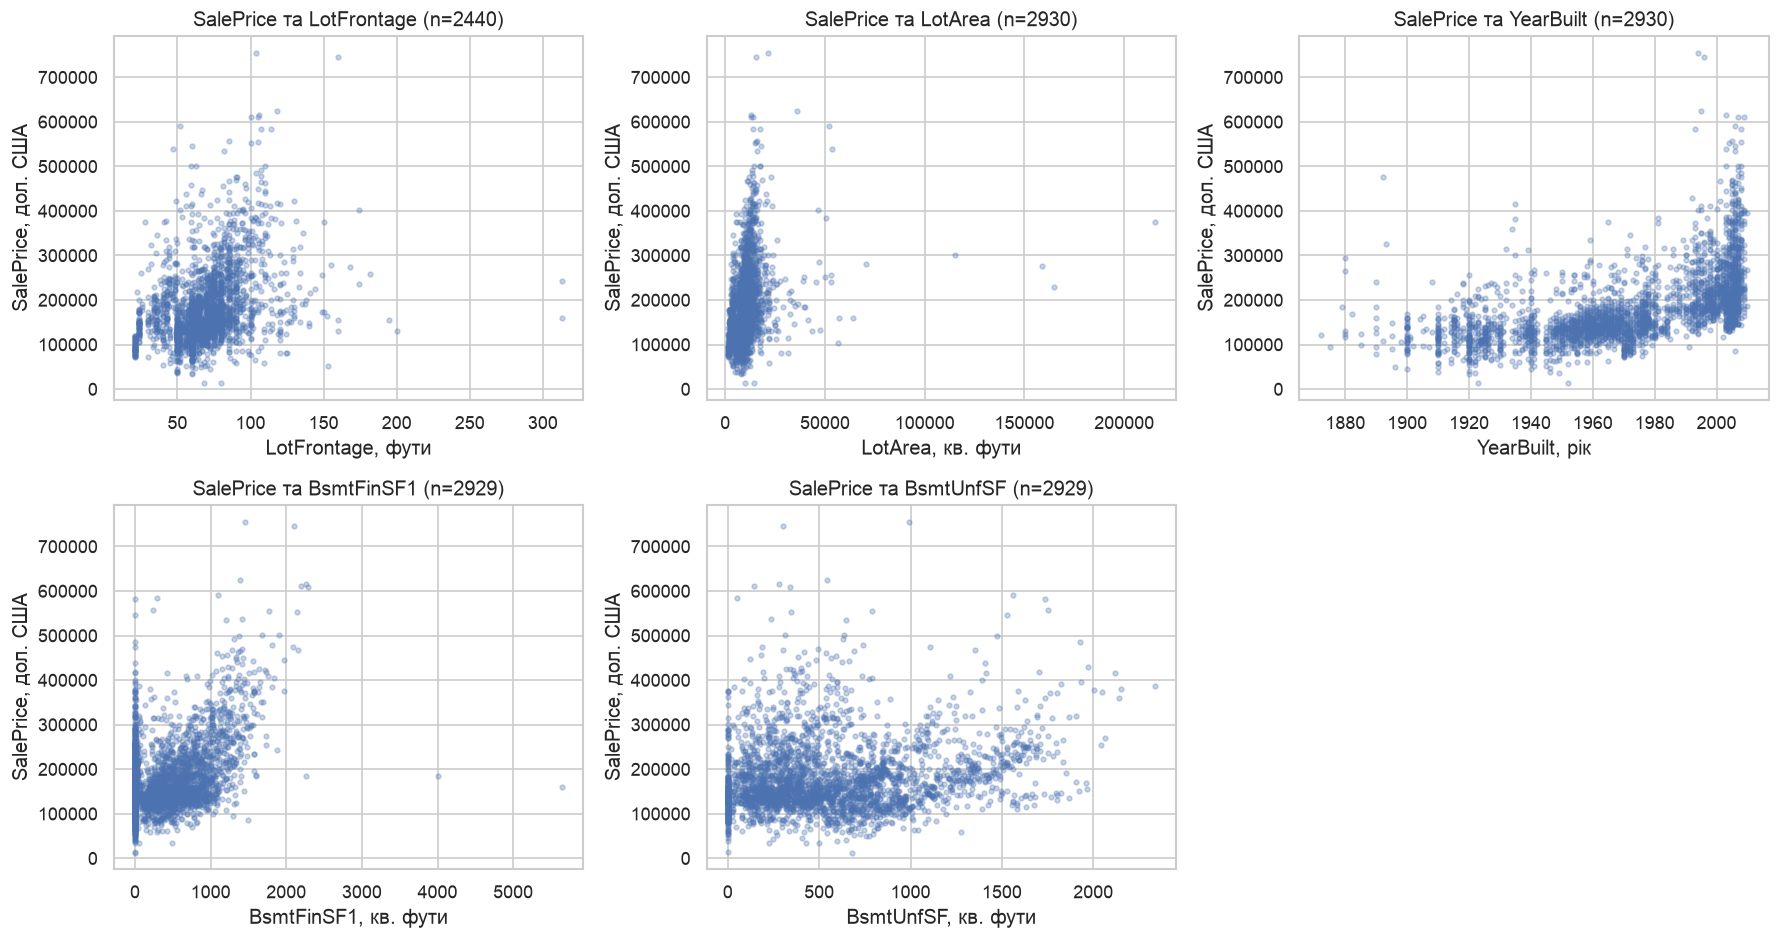
\includegraphics[width=\linewidth,height=0.82\textheight,keepaspectratio]{../../figures/problem5_scatter.png}
\caption{Ціна продажу та п'ять числових регресорів.}
\end{figure}


\answerheading
\begin{itemize}
\item
  LotFrontage (кореляція 0.357): ціна росте приблизно до 100 футів
  фасаду, далі зростання слабне; є кілька дуже широких ділянок (до 313
  футів). Можна спробувати \texttt{np.log(LotFrontage)} або квадратичний
  член. Також ця змінна має 490 пропусків.
\item
  LotArea (0.267): більшість ділянок менші за 20 тис. кв. футів, але є
  кілька величезних (до 215245). Розподіл сильно скошений праворуч; такі
  точки матимуть великий важіль. Ціна з площею росте дедалі повільніше,
  тому доречний \texttt{np.log(LotArea)}.
\item
  YearBuilt (0.558, найсильніший зв'язок): залежність опукла. Медіанна
  ціна: 119 тис. (до 1920 р.), 126 тис. (1921--1950), 143 тис.
  (1951--1980), 200 тис. (1981--2000), 226 тис. (після 2000). Для нових
  будинків більший і розкид (стандартне відхилення 73--88 тис. проти
  41--50 тис.). Можна додати \(YearBuilt^2\), вік будинку
  \texttt{YrSold\ -\ YearBuilt} або моделювати \texttt{log(SalePrice)}.
\item
  BsmtFinSF1 (0.433): 31.7\% нулів (немає обробленої площі підвалу),
  тому на графіку є вертикальна смуга біля 0. Для додатних значень
  зв'язок близький до лінійного. Дві точки з площею 4010 і 5644 мають
  низьку ціну (Order 2181 і 1499); це потенційні викиди. Розширення:
  індикатор \texttt{BsmtFinSF1\ \textgreater{}\ 0}.
\item
  BsmtUnfSF (0.183): слабкий зв'язок і великий розкид; 8.3\% нулів.
  Окремо ця площа мало пояснює; її краще розглядати разом з іншими
  площами підвалу.
\end{itemize}

На всіх графіках розкид цін зростає для дорожчих будинків
(гетероскедастичність), а сама ціна скошена праворуч. Це аргументи за
\texttt{np.log(SalePrice)}. Будинок Order 1499 крайній одразу за
кількома змінними. Далі за умовою спочатку оцінюємо просту модель без
трансформацій; специфікацію з логарифмом ціни розглянемо окремо.


\Needspace{225.0pt}

\subsection{(3) Проста лінійна регресія}

\begin{taskstatement}
Підгоніть просту лінійну регресію за допомогою класу OLS з бібліотеки
statsmodels без виконання обговорених вище трансформацій. Виберіть один
із числових регресорів, наприклад, LotArea. Запишіть відповідну гіпотезу
для t-тесту. Наведіть формулу для тест-статистики, поясніть компоненти
цієї формули та вкажіть значення для цих компонентів із регресійного
звіту (summary()). Оцініть якість підгонки (goodness-of-fit) моделі.
Поясніть своїми словами різницю між \(R^2\) та скоригованим (adjusted)
\(R^2\).
\end{taskstatement}


\pythoncode{p5-c11}

\Needspace{258.4pt}

\resulttext{p5-c11-out0.txt}

\begingroup\fontsize{7.5}{9.5}\selectfont\setlength{\tabcolsep}{2.5mm}\renewcommand{\arraystretch}{1.15}
\par\vspace{2pt}\noindent\begin{tabular}{|ll|}
\hline
 & Значення \\
\hline
n & 2930 \\
beta\_1 & 2.70224 \\
SE(beta\_1) & 0.180575 \\
t & 14.9646 \\
df = n - 2 & 2928 \\
p & 7.63384e-49 \\
t\_0.975,df & 1.96077 \\
R² & 0.0710485 \\
Скоригований R² & 0.0707312 \\
Стандартна похибка регресії, дол. & 77009.6 \\
\hline
\end{tabular}\par\vspace{2pt}
\endgroup


\answerheading
Модель: \(SalePrice_i=\beta_0+\beta_1 LotArea_i+\varepsilon_i\), де
\(\beta_0\) позначає вільний член, \(\beta_1\) нахил, \(\varepsilon_i\)
похибку продажу \(i\); \(n=2930\).

Гіпотези t-тесту: \(H_0:\beta_1=0\) (площа ділянки лінійно не пов'язана
з ціною) проти \(H_1:\beta_1\ne0\).

\[t=\frac{\widehat\beta_1-0}{SE(\widehat\beta_1)},\qquad SE(\widehat\beta_1)=\sqrt{\frac{\widehat\sigma^2}{\sum_i(x_i-\bar x)^2}},\qquad df=n-2.\]
де \(\widehat\beta_1\) позначає оцінку нахилу, \(SE(\widehat\beta_1)\)
її стандартну похибку, \(\widehat\sigma^2=RSS/(n-2)\) оцінку дисперсії
похибок, \(x_i\) значення \texttt{LotArea}, \(\bar x\) їх середнє, \(n\)
кількість спостережень, \(df\) кількість ступенів вільності.

Компоненти з \texttt{summary()}:

\begin{itemize}
\item
  \(\widehat\beta_1=2.7022\) (\texttt{coef}), оцінений нахил: +1 кв. фут
  ділянки відповідає в середньому +2.70 дол. ціни;
\item
  \(SE(\widehat\beta_1)=0.1806\) (\texttt{std\ err}), тобто наскільки
  оцінка коливалася б від вибірки до вибірки;
\item
  0, значення \(\beta_1\) за \(H_0\);
\item
  \(t=2.7022/0.1806=14.96\) (\texttt{t}), \(df=2928\)
  (\texttt{Df\ Residuals});
\item
  \(p=7.6\cdot10^{-49}\) (\texttt{P\textgreater{}\textbar{}t\textbar{}}
  показує 0.000).
\end{itemize}

\(|t|=14.96>t_{0.975,2928}=1.961\), тому \(H_0\) відхиляємо: площа
ділянки статистично значуща.

Якість підгонки слабка: \(R^2=0.071\), тобто площа ділянки пояснює лише
7.1\% варіації цін. Стандартна похибка регресії
\(\widehat\sigma=\sqrt{RSS/(n-2)}\) становить близько 77 тис. дол.: це
типовий розмір залишку. F-статистика 223.9 для однієї змінної дорівнює
\(t^2\). Значущий коефіцієнт ще не означає добру модель. Також
\texttt{summary()} показує ненормальні залишки (Jarque--Bera = 4394).
Великий \texttt{Cond.\ No.} тут пов'язаний лише з масштабом: значення
\texttt{LotArea} сягають десятків тисяч кв. футів, а константа дорівнює
1. З одним регресором мультиколінеарності немає.

\(R^2\) і скоригований \(R^2\):
\[R^2=1-\frac{RSS}{TSS},\qquad \bar R^2=1-\frac{RSS/(n-k)}{TSS/(n-1)}.\]
де \(RSS\) позначає суму квадратів залишків, \(TSS\) суму квадратів
відхилень ціни від її середнього, \(k\) кількість параметрів разом із
константою, \(n\) кількість спостережень.

\(R^2\) показує частку поясненої варіації; він ніколи не зменшується при
додаванні змінної, навіть зовсім шумової. Скори\-гований \(R^2\) штрафує
за кількість параметрів \(k\) і зростає лише тоді, коли нова змінна
достатньо зменшує RSS. Тут \(k=2\), тому різниця мізерна: 0.0710 проти
0.0707. Для повної моделі з 269 параметрами різниця вже помітна: 0.9399
проти 0.9324.


\Needspace{225.0pt}

\subsection{(4) Спільний F-тест для MSSubClass}

\begin{taskstatement}
Якщо ви хочете стверджувати, що змінна MSSubClass є незначущою, і
використовуєте модель із фіктивними змінними, то вам необхідно
перевірити одночасну (спільну) незначущість усіх даммі-змінних, що
походять від факторної змінної MSSubClass. Запустіть тест для загальної
лінійної гіпотези за допомогою методу f\_test() у statsmodels та зробіть
висновок про значущість MSSubClass. Запишіть матрицю та вектор, які
необхідні для формулювання цієї гіпотези в межах лінійної моделі.
\end{taskstatement}


\pythoncode{p5-c14}

\Needspace{56.0pt}

\resulttext{p5-c14-out0.txt}

\begingroup\fontsize{7.5}{9.5}\selectfont\setlength{\tabcolsep}{2.5mm}\renewcommand{\arraystretch}{1.15}
\par\vspace{2pt}\noindent\begin{tabular}{|ll|}
\hline
 & Спільний F-тест \\
\hline
F & 1.40493 \\
df1 = q & 13 \\
df2 = n - k & 2145 \\
p & 0.148857 \\
F\_0.95 & 1.72472 \\
RSS без MSSubClass & 1.01765e+12 \\
RSS повної моделі & 1.00905e+12 \\
\hline
\end{tabular}\par\vspace{2pt}
\endgroup


\answerheading
Повна модель має \(n=2414\), \(k=269\) параметрів: константу, 32 числові
регресори та 236 фіктивних змінних. \(R^2=0.9399\).

Для єдиного розв'язку МНК прибираємо точні лінійні залежності:
\texttt{TotalBsmtSF} і \texttt{GrLivArea} є сумами інших площ, а частина
фіктивних змінних збігається. При цьому важливо зберегти зміст змінних,
які контролюємо.

Особливість MSSubClass: у робочій вибірці є 15 класів, тобто 14
індикаторів відносно класу 20. Але \texttt{MSSubClass\_90} точно
збігається з \texttt{BldgType\_Duplex}. Якщо ми перевіряємо внесок
MSSubClass понад усі інші змінні, індикатор дуплексу має залишатися в
обох моделях. Тому залишаємо його під назвою \texttt{BldgType\_Duplex},
а для MSSubClass маємо 13 незалежних обмежень. Єдиний продаж класу 150
не входить у робочу вибірку через пропущений \texttt{LotFrontage}.

Гіпотеза: \(H_0\): усі 13 окремо оцінюваних коефіцієнтів MSSubClass
дорівнюють нулю; \(H_1\): хоча б один не дорівнює нулю. У матричному
вигляді:
\[H_0:R\beta=r,\qquad R=\big[\,0_{13\times37}\;|\;I_{13}\;|\;0_{13\times219}\,\big],\qquad r=0_{13}.\]
Тут \(\beta\) позначає вектор 269 коефіцієнтів повної моделі, \(R\)
матрицю обмежень розміру \(13\times269\), \(I_{13}\) одиничну матрицю,
\(0_{13\times37}\) і \(0_{13\times219}\) нульові блоки, \(r\) нульовий
вектор довжини 13. У порядку \texttt{X\_full} перед MSSubClass стоять
константа, 32 числові регресори й 4 індикатори BldgType. Одиниці \(R\)
вибирають стовпці 37--49 (індексація від 0), як показує вивід коду.

\texttt{f\_test()} перевіряє ці обмеження. Той самий результат
отримуємо, порівнюючи моделі з MSSubClass і без нього, але з усіма
іншими змінними в обох:
\[F=\frac{(RSS_R-RSS_U)/13}{RSS_U/(2414-269)}=1.405,\qquad p=0.149.\] де
\(RSS_R\) позначає суму квадратів залишків обмеженої моделі без
MSSubClass, \(RSS_U\) повної моделі, 13 кількість обмежень, \(2414-269\)
кількість ступенів вільності залишків повної моделі.

На рівні 0.05 не відхиляємо \(H_0\): дані не дають достатніх доказів, що
MSSubClass додає пояснення ціни після врахування BldgType, HouseStyle,
YearBuilt та решти регресорів. Це не доводить відсутності будь-якого
зв'язку типу житла з ціною: частину інформації вже містять інші змінні.

Це класичний F-тест за припущення однакової дисперсії та нормальності
похибок; якщо вони порушені, p-значення є лише наближеним.


\Needspace{199.0pt}

\subsection{(5) Інтерпретація коефіцієнтів}

\begin{taskstatement}
Дайте економічну інтерпретацію параметрів для LotArea, першої фіктивної
змінної для MSSubClass (це підступне питання!) та BedroomAbvGr.
(Ігноруйте потенційну незначущість коефіцієнтів.) Як зміниться
інтерпретація, якщо моделювати логарифм від SalePrice
(np.log(df{[}`SalePrice'{]})), використовуючи лог-лінійну специфікацію?
\end{taskstatement}


\pythoncode{p5-c17}

\begingroup\fontsize{7.5}{9.5}\selectfont\setlength{\tabcolsep}{1.5mm}\renewcommand{\arraystretch}{1.15}
\par\vspace{2pt}\noindent\begin{tabular}{|>{\raggedright\arraybackslash}p{21.32mm}>{\raggedright\arraybackslash}p{28.47mm}>{\raggedright\arraybackslash}p{21.32mm}>{\raggedright\arraybackslash}p{27.75mm}>{\raggedright\arraybackslash}p{20.40mm}>{\raggedright\arraybackslash}p{27.75mm}|}
\hline
 & beta (Sale\allowbreak{}Price), дол. & p (Sale\allowbreak{}Price) & gamma (log Sale\allowbreak{}Price) & 100*gamma, \% & 100*(exp(gamma)-1), \% \\
\hline
LotArea & 0.798701 & 5.71237e-13 & 3.06586e-06 & 0.000306586 & 0.000306587 \\
MSSubClass\_30 & 5508.22 & 0.0913135 & -0.0413429 & -4.13429 & -4.05 \\
BedroomAbvGr & -3263.73 & 0.000872302 & -0.00100473 & -0.100473 & -0.100423 \\
\hline
\end{tabular}\par\vspace{2pt}
\endgroup


\Needspace{28.4pt}

\resulttext{p5-c17-out1.txt}

\begingroup\fontsize{7.5}{9.5}\selectfont\setlength{\tabcolsep}{2.5mm}\renewcommand{\arraystretch}{1.15}
\par\vspace{2pt}\noindent\begin{tabular}{|llll|}
\hline
MSSub\allowbreak{}Class & count & min & max \\
\hline
20 & 881 & 1938 & 2010 \\
30 & 126 & 1885 & 1948 \\
\hline
\end{tabular}\par\vspace{2pt}
\endgroup


\answerheading
Усі інтерпретації подано за незмінних інших змінних повної моделі.

Модель для \texttt{SalePrice} (у доларах):

\begin{itemize}
\item
  LotArea: \(\widehat\beta=0.80\). Додатковий кв. фут ділянки відповідає
  в середньому +0.80 дол., а +1000 кв. футів дають +799 дол. Це значно
  менше, ніж 2.70 у простій регресії (пункт 3): там \texttt{LotArea}
  частково відображала розмір будинку, район тощо.
\item
  Перша фіктивна \texttt{MSSubClass\_30}: \(\widehat\beta=5508\).
  Підступ у тому, що це не ефект «збільшення коду на одиницю» і не ціна
  класу 30. Це різниця з базовим класом 20: будинок класу 30
  (одноповерховий, 1945 р. і старший) у середньому на 5.5 тис. дол.
  дорожчий за будинок класу 20 (одноповерховий, 1946 р. і новіший) за
  інших рівних. Інша база дала б інший коефіцієнт. Крім того, класи 20 і
  30 визначено через рік побудови, а \texttt{YearBuilt} уже є в моделі.
  «Однаковий рік» для двох класів трапляється рідко: у вибірці клас 30
  збудовано у 1885--1948 рр., а клас 20 у 1938--2010 рр. Коефіцієнт
  оцінено на всій вибірці, але перекриття років між класами обмежене,
  тому порівняння «за однакового року» сильно залежить від лінійної
  форми моделі. За звичайним t-тестом він незначущий на рівні 0.05
  (\(p=0.09\)). Проста різниця середніх у пункті 1 була \(-90.6\) тис.,
  бо вона включала й вік, і розмір будинку.
\item
  BedroomAbvGr: \(\widehat\beta=-3264\). Ще одна спальня за тих самих
  площ поверхів відповідає ціні, нижчій у середньому на 3.3 тис. дол.:
  та сама площа ділиться на більше дрібних кімнат. Без контролю площі
  зв'язок кількості спалень із ціною був би додатним.
\end{itemize}

Лог-лінійна модель \(\log(SalePrice)=X\gamma+u\), де \(X\) позначає ту
саму матрицю регресорів, \(\gamma\) вектор коефіцієнтів, \(u\) похибку:
коефіцієнт \(\gamma_j\) показує зміну логарифма ціни. Тоді ціна
змінюється приблизно на \(100\gamma_j\%\), а точно на
\(100(e^{\gamma_j}-1)\%\):

\begin{itemize}
\item
  LotArea: \(\widehat\gamma=3.07\cdot10^{-6}\), тобто +1000 кв. футів
  дають приблизно +0.31\% ціни;
\item
  MSSubClass\_30: \(\widehat\gamma=-0.0413\), тобто клас 30 приблизно на
  4.1\% (точно на 4.05\%) дешевший за клас 20. Знак відрізняється від
  моделі ціни в доларах: ці дві специфікації по-різному описують
  залежність ціни від ознак.
\item
  BedroomAbvGr: \(\widehat\gamma=-0.0010\), тобто приблизно \(-0.10\%\)
  на спальню.
\end{itemize}

У лог-моделі ефекти відсоткові, а не в доларах: та сама зміна регресора
дає більше доларів для дорожчого будинку. Для фіктивних змінних із
великим \(\gamma\) варто брати точну формулу \(100(e^{\gamma}-1)\%\). Ці
відсотки описують зміну прогнозу \(e^{X\gamma}\), тобто умовної медіани
ціни за симетричних похибок. Для середньої ціни потрібне ще припущення,
що множник \(E[e^{u}\mid X]\) не залежить від \(X\).


\Needspace{238.0pt}

\subsection{(6) Довірчий інтервал і нормальність}

\begin{taskstatement}
Обчисліть 95\% довірчий інтервал для параметра LotArea (використовуючи
метод conf\_int()) та поясніть його економічний зміст. Зв'яжіть довірчі
інтервали з тестами значущості, тобто поясніть, як би ви використовували
ці інтервали для прийняття рішення про значущість відповідних
пояснювальних змінних? Довірчі інтервали обчислюються на основі
припущення, що залишки (residuals) підпорядковуються нормальному
розподілу. Чи виконується це припущення? Запустіть відповідний критерій
згоди за допомогою scipy.stats.shapiro або jarque\_bera.
\end{taskstatement}


\pythoncode{p5-c20}

\begin{figure}[H]
\centering
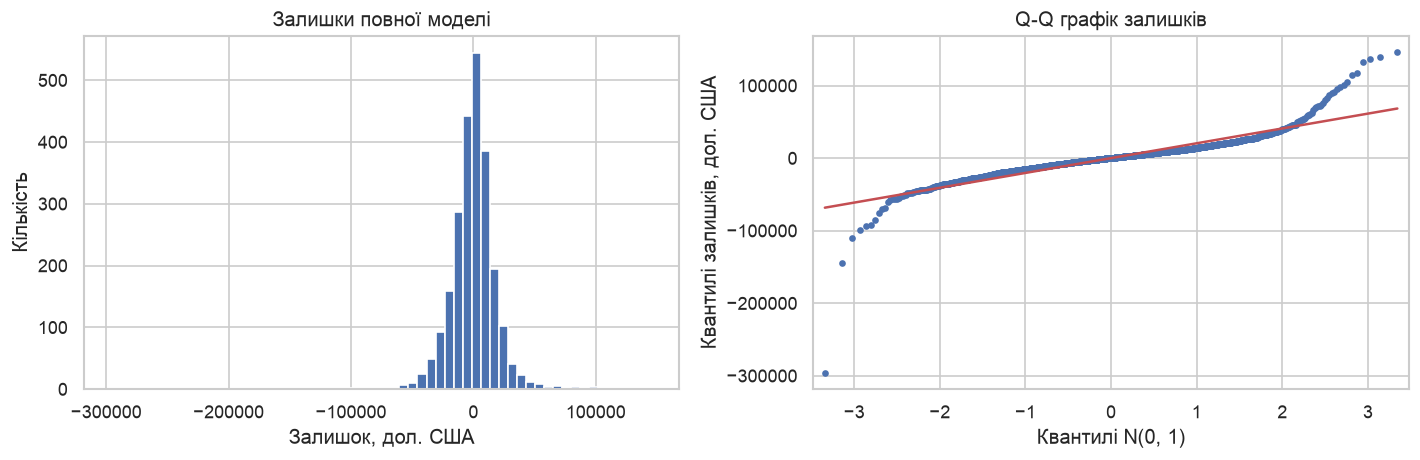
\includegraphics[width=\linewidth,height=0.82\textheight,keepaspectratio]{../../figures/problem5_normality.png}
\caption{Розподіл і Q-Q графік залишків повної моделі.}
\end{figure}


\begingroup\fontsize{7.5}{9.5}\selectfont\setlength{\tabcolsep}{2.5mm}\renewcommand{\arraystretch}{1.15}
\par\vspace{2pt}\noindent\begin{tabular}{|ll|}
\hline
 & Lot\allowbreak{}Area, повна модель \\
\hline
beta\_LotArea & 0.798701 \\
SE & 0.110137 \\
t\_0.975,n-k & 1.96107 \\
Нижня межа & 0.582715 \\
Верхня межа & 1.01469 \\
p t-тесту & 5.71237e-13 \\
\hline
\end{tabular}\par\vspace{2pt}
\endgroup


\begingroup\fontsize{7.5}{9.5}\selectfont\setlength{\tabcolsep}{2.5mm}\renewcommand{\arraystretch}{1.15}
\par\vspace{2pt}\noindent\begin{tabular}{|ll|}
\hline
 & Jarque-Bera для залишків \\
\hline
JB & 66037.7 \\
p & 0 \\
Асиметрія & -0.595274 \\
Ексцес (нормальний = 3) & 28.5955 \\
\hline
\end{tabular}\par\vspace{2pt}
\endgroup


\clearpage

\answerheading
95\% довірчий інтервал для \(\beta_{LotArea}\) у повній моделі:
\[\widehat\beta\pm t_{0.975,\,n-k}\,SE(\widehat\beta)=0.7987\pm1.961\cdot0.1101=[0.583;\;1.015]\ \text{дол. за кв. фут}.\]
де \(\widehat\beta\) позначає оцінку коефіцієнта, \(SE(\widehat\beta)\)
її стандартну похибку, \(t_{0.975,\,n-k}\) квантиль t-розподілу з
\(n-k=2145\) ступенями вільності.

Економічний зміст: за інших рівних додаткові 1000 кв. футів ділянки
пов'язані зі зростанням середньої ціни приблизно на 583--1015 дол. Число
«95\%» стосується процедури: якби ми багато разів брали нові вибірки й
будували інтервал так само, близько 95\% інтервалів накрили б справжнє
\(\beta\) (якщо припущення моделі виконуються). Це інтервал для
коефіцієнта, а не для ціни окремого будинку.

Зв'язок із тестом: двосторонній t-тест \(H_0:\beta=\beta_0\) на рівні
\(\alpha\) відхиляє \(H_0\) тоді й лише тоді, коли \(\beta_0\) не
потрапляє в \((1-\alpha)\)-інтервал. Для значущості беремо
\(\beta_0=0\). Тут 0 лежить поза \([0.583;\,1.015]\), тому
\texttt{LotArea} значуща на рівні 0.05 (\(p=5.7\cdot10^{-13}\)).
Інтервал дає більше, ніж p-значення: він показує ще й правдоподібний
розмір ефекту.

Нормальність залишків. Тест Jarque--Bera:
\(JB=\frac n6\big(S^2+\frac{(K-3)^2}4\big)\), де \(n\) позначає
кількість залишків, \(S\) їхню асиметрію, \(K\) ексцес (куртозис);
\(H_0\): розподіл нормальний. Отримали \(JB=66038\), \(p\approx0\)
(менше за точність обчислень). Асиметрія \(-0.60\), ексцес 28.6 (у
нормального 3): хвости дуже важкі. На Q--Q графіку крайні точки далеко
від прямої, окремі залишки сягають \(-300\) тис. дол. Припущення
нормальності не виконується.

Тому точні t-інтервали тут лише наближення. Для \(n=2414\) вони
залишаються наближено правильними, якщо інші припущення (незалежність,
однаковий розкид похибок) виконуються. Проте гістограма та Q--Q графік
показують важкі хвости й кілька дуже великих залишків. Тому стандартні
похибки й інтервали слід сприймати обережно.


\clearpage

\Needspace{225.0pt}

\subsection{(7) Покроковий відбір за BIC}

\begin{taskstatement}
Більшість змінних можуть виявитися незначущими, тому нам слід знайти
найменшу (найбільш економну) модель, яка все ще має хорошу пояснювальну
здатність. Виберіть таку модель за допомогою покрокового відбору змінних
(stepwise model selection), реалізувавши власний алгоритм на основі
метрик AIC/BIC або скориставшись методами регуляризації Lasso з
sklearn.linear\_model. Детально поясніть, як цей метод/підхід працює у
вашому коді. Працюйте з цією обраною моделлю на всіх наступних кроках.
\end{taskstatement}


\pythoncode{p5-c23}

\begingroup\fontsize{7.5}{9.5}\selectfont\setlength{\tabcolsep}{2.5mm}\renewcommand{\arraystretch}{1.15}
\par\vspace{2pt}\noindent\begin{tabular}{|llll|}
\hline
Крок & Вилучено & k & BIC \\
\hline
0 & - & 269 & 56866.2 \\
1 & Exterior2nd & 254 & 56759.9 \\
2 & MSSubClass & 241 & 56679.4 \\
3 & Exterior1st & 226 & 56606.7 \\
4 & SaleType & 217 & 56546 \\
… & … & … & … \\
44 & GarageFinish & 95 & 55905.8 \\
45 & Street & 94 & 55902.6 \\
46 & HalfBath & 93 & 55900.6 \\
47 & KitchenAbvGr & 92 & 55898.9 \\
48 & YearRemodAdd & 91 & 55897.5 \\
\hline
\end{tabular}\par\nopagebreak\vspace{-1pt}{\itshape\color{black!60}Скорочено: з 49 рядків історії показано кроки 0–4 і 44–48; рядок «…» позначає пропущені кроки 5–43.}
\par\vspace{2pt}
\endgroup


\Needspace{46.8pt}

\resulttext{p5-c23-out1.txt}

\begingroup\fontsize{7.5}{9.5}\selectfont\setlength{\tabcolsep}{2.5mm}\renewcommand{\arraystretch}{1.15}
\par\vspace{2pt}\noindent\begin{tabular}{|lllllll|}
\hline
 & Змінних & Параметрів k & R² & Скоригований R² & AIC & BIC \\
\hline
Повна & 76 & 269 & 0.939889 & 0.932378 & 55308.9 & 56866.2 \\
Після відбору & 28 & 91 & 0.928533 & 0.925764 & 55370.7 & 55897.5 \\
\hline
\end{tabular}\par\vspace{2pt}
\endgroup


\answerheading
Використано власний зворотний покроковий відбір за BIC:
\[BIC=-2\ln\widehat L+k\ln n,\qquad -2\ln\widehat L=n\ln(RSS/n)+\text{const}.\]
Тут \(\widehat L\) позначає максимум функції правдоподібності, \(k\)
кількість незалежних параметрів разом із константою, \(n\) кількість
спостережень, \(RSS\) суму квадратів залишків. Для \(n=2414\) штраф за
параметр \(\ln n\approx7.8\), а в AIC лише 2. BIC сильніше штрафує
складність.

Як працює код:

\begin{enumerate}
\def\labelenumi{\arabic{enumi}.}
\item
  Починаємо з усіх 76 початкових регресорів: 32 числових і 44
  категоріальних.
\item
  Для кожного можливого вилучення заново будуємо матрицю з повних блоків
  решти початкових змінних та прибираємо дубльовані стовпці лише в цій
  кандидатній моделі.
\item
  Оцінюємо моделі та вилучаємо змінну, без якої BIC найменший, якщо це
  покращує поточний BIC.
\item
  Повторюємо до зупинки.
\end{enumerate}

Категоріальну змінну розглядаємо цілком. Якщо два фактори мають спільний
індикатор, він залишається, доки потрібен хоча б одному з них.
Наприклад, після вилучення MSSubClass у моделі лишається
\texttt{BldgType\_Duplex}. Так само відновлюються потрібні індикатори
відсутності підвалу чи гаража. Тому відбір стосується початкових
змінних, а не довільного розподілу спільних стовпців між ними. Усі
моделі використовують ті самі 2414 рядків.

Результат: за 48 кроків вилучено 48 регресорів, залишилося 28 змінних і
91 параметр. Серед них площі, рік будівництва, кількість спалень і
ванних кімнат, якість будинку, тип будівлі та район. Повний список і
скорочену історію кроків наведено у виводі коду.

Обрана модель має майже втричі менше параметрів, втрачає приблизно 0.011
у \(R^2\), а BIC зменшується приблизно на 969. AIC із цих двох моделей
віддає перевагу повній, бо слабше штрафує складність. Покроковий відбір
перевіряє не всі комбінації, тому не гарантує глобально найменшого BIC.

У вибраній моделі лишилися рідкісні категорії (\texttt{RoofMatl},
\texttt{PoolQC}, \texttt{MiscFeature} тощо). Їхню роль варто перевірити
через важіль і відстань Кука, а якість прогнозів через крос-валідацію.


\Needspace{238.0pt}

\subsection{(8) Викиди, важіль і вплив}

\begin{taskstatement}
Іноді дані містять викиди (outliers), що спричиняє зсув в оцінках
параметрів. Перевірте наявність викидів за допомогою графіків залишків,
відстані Кука (Cook's distance) та важеля (leverage). Для обчислення цих
показників скористайтеся класом OLSInfluence з бібліотеки statsmodels.
Зверніть прискіпливу увагу на спостереження з найбільшим значенням
важеля (leverage). Що саме робить це спостереження таким видатним (ви
можете побудувати sns.boxplot для інтервальних змінних або порахувати
частоти через value\_counts())?
\end{taskstatement}


\pythoncode{p5-c26}

\Needspace{28.4pt}

\resulttext{p5-c26-out0.txt}

\begingroup\fontsize{7.5}{9.5}\selectfont\setlength{\tabcolsep}{2.5mm}\renewcommand{\arraystretch}{1.15}
\par\vspace{2pt}\noindent\begin{tabular}{|lllll|}
\hline
Order & Sale\allowbreak{}Price & h & Залишок & Рідкісні рівні (кількість продажів) \\
\hline
211 & 107500 & 1 & 3.31056e-08 & KitchenQual=Po (1) \\
1402 & 241500 & 1 & 5.76838e-08 & RoofMatl=Membran (1) \\
1499 & 160000 & 1 & 9.62755e-08 & RoofMatl=ClyTile (1) \\
1908 & 137000 & 1 & 3.45754e-08 & RoofMatl=Roll (1) \\
2181 & 183850 & 1 & 5.73054e-08 & MiscFeature=Elev (1) \\
2299 & 80000 & 1 & 5.13101e-08 & MasVnrType=CBlock (1) \\
2351 & 250000 & 1 & 1.55123e-08 & PoolQC=Fa (2), MiscFeature=TenC (1) \\
2358 & 181000 & 1 & 2.90456e-08 & PoolQC=Fa (2) \\
\hline
\end{tabular}\par\vspace{2pt}
\endgroup


\Needspace{28.4pt}

\resulttext{p5-c26-out2.txt}

\begingroup\fontsize{7.5}{9.5}\selectfont\setlength{\tabcolsep}{1.5mm}\renewcommand{\arraystretch}{1.15}
\par\vspace{2pt}\noindent\begin{tabular}{|>{\raggedright\arraybackslash}p{11.52mm}>{\raggedright\arraybackslash}p{18.64mm}>{\raggedright\arraybackslash}p{19.48mm}>{\raggedright\arraybackslash}p{14.91mm}>{\raggedright\arraybackslash}p{15.91mm}>{\raggedright\arraybackslash}p{13.86mm}>{\raggedright\arraybackslash}p{13.86mm}>{\raggedright\arraybackslash}p{14.91mm}>{\raggedright\arraybackslash}p{14.91mm}|}
\hline
Order & Neighbor\-hood & Sale\allowbreak{}Condition & 1st\allowbreak{}Flr\allowbreak{}SF & Sale\allowbreak{}Price & Прогноз & Залишок & h & Cook\_D \\
\hline
2182 & Edwards & Partial & 3138 & 184750 & 489336 & -304586 & 0.294699 & 1.16948 \\
514 & Somerst & Normal & 2490 & 468000 & 324780 & 143220 & 0.269261 & 0.220088 \\
1761 & NoRidge & Abnorml & 2411 & 745000 & 625485 & 119515 & 0.291387 & 0.176375 \\
2571 & NAmes & Abnorml & 1360 & 235000 & 344412 & -109412 & 0.279098 & 0.136797 \\
1015 & StoneBr & Normal & 1710 & 334000 & 239299 & 94701 & 0.281954 & 0.104358 \\
\hline
\end{tabular}\par\vspace{2pt}
\endgroup


\begingroup\fontsize{7.5}{9.5}\selectfont\setlength{\tabcolsep}{1.5mm}\renewcommand{\arraystretch}{1.15}
\par\vspace{2pt}\noindent\begin{tabular}{|>{\raggedright\arraybackslash}p{15.71mm}>{\raggedright\arraybackslash}p{8.59mm}>{\raggedright\arraybackslash}p{13.90mm}>{\raggedright\arraybackslash}p{14.52mm}>{\raggedright\arraybackslash}p{10.33mm}>{\raggedright\arraybackslash}p{11.12mm}>{\raggedright\arraybackslash}p{11.12mm}>{\raggedright\arraybackslash}p{11.86mm}>{\raggedright\arraybackslash}p{11.86mm}>{\raggedright\arraybackslash}p{11.12mm}>{\raggedright\arraybackslash}p{11.86mm}|}
\hline
 & Order & Neighbor\-hood & Sale\allowbreak{}Condition & Lot\allowbreak{}Area & 1st\allowbreak{}Flr\allowbreak{}SF & 2nd\allowbreak{}Flr\allowbreak{}SF & Year\allowbreak{}Built & Sale\allowbreak{}Price & h & Cook\_D \\
\hline
2180 & 2181 & Edwards & Partial & 39290 & 5095 & 0 & 2008 & 183850 & 1 & NaN \\
1498 & 1499 & Edwards & Partial & 63887 & 4692 & 950 & 2008 & 160000 & 1 & NaN \\
2181 & 2182 & Edwards & Partial & 40094 & 3138 & 1538 & 2007 & 184750 & 0.294699 & 1.16948 \\
956 & 957 & Timber & Normal & 215245 & 2036 & 0 & 1965 & 375000 & 0.662552 & 0.0219219 \\
Медіана вибірки & NaN & NaN & NaN & 9245.5 & 1073 & 0 & 1972 & 157000 & NaN & NaN \\
\hline
\end{tabular}\par\vspace{2pt}
\endgroup


\begin{figure}[H]
\centering
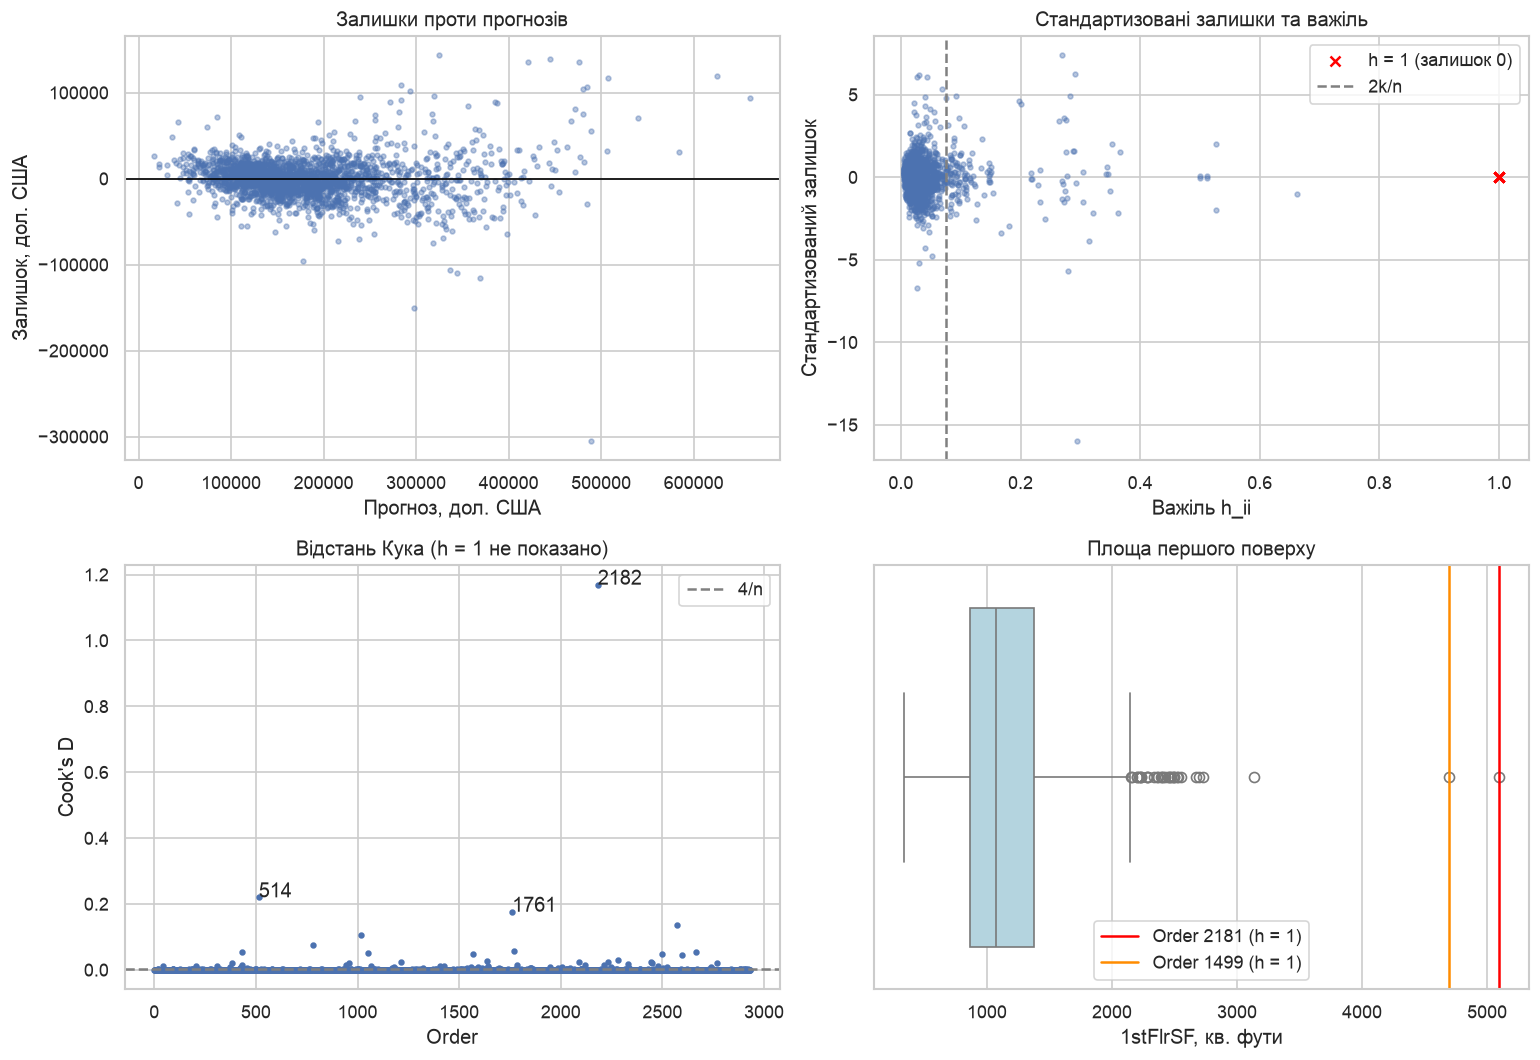
\includegraphics[width=\linewidth,height=0.82\textheight,keepaspectratio]{../../figures/problem5_influence.png}
\caption{Залишки, важіль, відстань Кука та нетипові площі.}
\end{figure}


\begingroup\fontsize{7.5}{9.5}\selectfont\setlength{\tabcolsep}{2.5mm}\renewcommand{\arraystretch}{1.15}
\par\vspace{2pt}\noindent\begin{tabular}{|lll|}
\hline
 & Усі продажі & Без Order 2182 \\
\hline
LotArea & 0.803024 & 0.932567 \\
1stFlrSF & 48.6615 & 51.9886 \\
2ndFlrSF & 55.525 & 60.1981 \\
BsmtFinSF1 & 42.6449 & 44.7811 \\
OverallQual & 6978.72 & 6976.48 \\
BedroomAbvGr & -4143.96 & -5228.88 \\
\hline
\end{tabular}\par\vspace{2pt}
\endgroup


\answerheading
Важіль \(h_{ii}\) є діагоналлю матриці \(H=X(X^TX)^{-1}X^T\), де \(X\)
позначає матрицю регресорів відібраної моделі. Він залежить лише від
регресорів і показує, наскільки незвичний набір ознак будинку. Маємо
\(0\le h_{ii}\le1\), \(\sum_i h_{ii}=k=91\). Середній важіль
\(k/n=0.0377\), орієнтир для великого важеля \(2k/n=0.0754\) перевищують
163 продажі.

Відстань Кука поєднує залишок і важіль:
\[D_i=\frac{e_i^2}{k\,s^2}\frac{h_{ii}}{(1-h_{ii})^2}.\] де \(e_i\)
позначає залишок спостереження \(i\), \(s^2=RSS/(n-k)\) оцінку дисперсії
похибок, \(k\) кількість параметрів. Вона вимірює зміну підгонки після
вилучення спостереження. Значення \(4/n\) і 1 є діагностичними
орієнтирами, а не автоматичними правилами видалення даних.

Найбільший важіль \(h=1\) мають 8 продажів. Причина в рідкісних
категоріях. Наприклад, Order 1499 є єдиним продажем із
\texttt{RoofMatl=ClyTile}, а Order 2181 із \texttt{MiscFeature=Elev}.
Order 2358 має \texttt{PoolQC=Fa}: таких продажів два, але інший уже
виділено унікальним індикатором \texttt{TenC}. Комбінація цих
індикаторів дозволяє точно підлаштувати обидва продажі. Залишки в усіх
восьми точках практично нульові; для \(h=1\) стандартна формула Кука не
визначена, тому показуємо \texttt{NaN}, а не помилковий нуль.

Особливо незвичні Order 1499 і 2181: будинки 2008 року в Edwards із
площами першого поверху 4692 та 5095 кв. футів за медіани 1073. Їхні
ціни становлять лише 160000 і 183850 дол. Обидва мають
\texttt{SaleCondition=Partial}: будинок не був завершений під час
останньої оцінки, згідно з описом даних. Рідкісні індикатори даху
ClyTile та ліфта Elev дозволяють моделі точно підігнати ці продажі.

Серед \(h<1\) найбільший важіль має Order 957, \(h=0.663\): ділянка
215245 кв. футів, приблизно у 23 рази більша за медіану. Проте його
відстань Кука \(D=0.022\) значно менша, ніж у найвпливовіших точок.
Великий важіль сам по собі не означає великої відстані Кука.

Найбільша визначена відстань Кука в Order 2182: \(D=1.17\), \(h=0.295\).
Фактична ціна 184750 дол., прогноз 489336 дол., залишок приблизно
\(-305\) тис. Без цього продажу коефіцієнт LotArea змінюється з 0.803 на
0.933, BedroomAbvGr з \(-4144\) на \(-5229\). Це показує чутливість
оцінок.

На графіку залишків розкид загалом більший для високих прогнозів, що
вказує на можливу гетероскедастичність. У даних є незвичні й впливові
продажі; автоматично їх не вилучаємо. Варто враховувати чутливість
висновків, а для покращення прогнозів дослідити великі будинки
\texttt{Partial} та об'єднання рідкісних рівнів категорій.


\Needspace{251.0pt}

\subsection{(9) Імпутація пропусків}

\begin{taskstatement}
Часто в даних трапляються пропуски. Виберіть 5 випадкових рядків у
наборі даних і видаліть значення для LotArea. Реалізуйте щонайменше два
підходи для заповнення (імпутації) цих значень за допомогою інструментів
pandas або класу SimpleImputer / IterativeImputer з sklearn.impute.
Запишіть відповідні формули/модель та наведіть мотивацію для вашого
підходу. Зауважте, що для імпутації слід використовувати повний набір
даних, а не лише набір змінних після відбору ознак. Зверніть увагу: ваш
алгоритм має обробляти лише дійсні пропуски (як-от у LotFrontage або
ваші штучні пропуски в LotArea), а не структурні категорії NA, які ви
мали зберегти як окремі факторні рівні.
\end{taskstatement}


\pythoncode{p5-c29}

\Needspace{37.599999999999994pt}

\resulttext{p5-c29-out0.txt}

\begingroup\fontsize{7.5}{9.5}\selectfont\setlength{\tabcolsep}{2.5mm}\renewcommand{\arraystretch}{1.15}
\par\vspace{2pt}\noindent\begin{tabular}{|lllll|}
\hline
Order & Neighbor\-hood & Справжня Lot\allowbreak{}Area & Медіана & Iterative\allowbreak{}Imputer \\
\hline
2266 & Timber & 13758 & 9434 & 6488.77 \\
1286 & OldTown & 10440 & 9434 & 8673.19 \\
1917 & NAmes & 8760 & 9434 & 9665.54 \\
262 & CollgCr & 10650 & 9434 & 12519.2 \\
1269 & NAmes & 7200 & 9434 & 7612.11 \\
\hline
\end{tabular}\par\vspace{2pt}
\endgroup


\begingroup\fontsize{7.5}{9.5}\selectfont\setlength{\tabcolsep}{2.5mm}\renewcommand{\arraystretch}{1.15}
\par\vspace{2pt}\noindent\begin{tabular}{|lll|}
\hline
 & MAE, кв. фути & Медіана |помилки|, кв. фути \\
\hline
Медіана & 1890.8 & 1216 \\
IterativeImputer & 2444.58 & 1766.81 \\
\hline
\end{tabular}\par\vspace{2pt}
\endgroup


\Needspace{28.4pt}

\resulttext{p5-c29-out3.txt}

\answerheading
Пропуски створено в копії повного \texttt{df} (2930 рядків, усі
колонки). П'ять випадкових рядків вибрано через \texttt{rng} із
\texttt{SEED\ =\ 42}: Order 2266, 1286, 1917, 262, 1269. Справжні
значення збережено лише для перевірки.

Що вважаємо пропуском: лише \texttt{NaN} у числових колонках. Це
справжні пропуски \texttt{LotFrontage} (490), \texttt{MasVnrArea} (23),
кілька пропусків у колонках підвалу й гаража та наші 5 штучних у
\texttt{LotArea}. Не чіпаємо:

\begin{itemize}
\item
  категоріальні \texttt{"NA"} (немає алеї, басейну, підвалу\ldots). Це
  окремі рівні, а не пропуски; \texttt{keep\_default\_na=False} зберіг
  їх як текст;
\item
  \texttt{GarageYrBlt} будинків без гаража: такого року не існує;
\item
  \texttt{SalePrice} (відгук, який потім пояснюємо) і
  \texttt{MSSubClass} (коди категорій).
\end{itemize}

Імпутація використовує 34 числові колонки.

Підхід 1, медіана (\texttt{SimpleImputer(strategy="median")}):
\[\widehat x_i=\operatorname{median}\{x_j:\ x_j\ \text{спостережено}\}.\]
де \(\widehat x_i\) позначає заповнене значення, \(x_j\) спостережені
значення тієї самої колонки. Для \texttt{LotArea} це 9434 кв. фути, для
\texttt{LotFrontage} 68 футів. Медіана проста й не залежить від кількох
дуже великих ділянок, які сильно змістили б середнє. Але всі пропуски
отримують одне значення, а інші ознаки будинку ігноруються.

Підхід 2, \texttt{IterativeImputer}: кожну колонку з пропусками по черзі
прогнозуємо лінійною регресією на всі інші колонки:
\[\widehat x_{i,LotArea}=b_0+\sum_j b_j x_{ij}.\] де \(x_{ij}\) позначає
значення інших числових колонок рядка \(i\), \(b_0\) і \(b_j\)
коефіцієнти регресії \texttt{LotArea} на них. Спочатку пропуски
заповнюються середніми, далі значення уточнюються раунд за раундом (до
25 раундів), доки зміни не стануть малими. Модель за замовчуванням
\texttt{BayesianRidge}, тобто лінійна регресія з невеликим штрафом на
коефіцієнти. Мотивація: площа ділянки пов'язана з фасадом, площею
будинку, гаражем тощо. Тому імпутацію робимо на повному наборі, а не
лише на змінних після відбору: інші змінні містять інформацію про
пропущене значення.

Результат на 5 прихованих значеннях: середня абсолютна помилка (MAE)
медіани становить 1891 кв. фут, \texttt{IterativeImputer} 2445. Тут
проста медіана виявилася точнішою; регресійний метод найбільше помилився
для Order 2266 (13758 \ensuremath{\rightarrow} 6489). П'яти значень замало для загального
висновку. Можлива причина: лінійна модель на початковій шкалі погано
описує скошену \texttt{LotArea}; варто було б імпутувати
\(\log(LotArea)\).

Обидва методи дають одне «найкраще» значення й не показують
невизначеності пропуску; медіана ще й зменшує розкид змінної. Подальші
регресії продовжуємо на тих самих 2414 повних спостереженнях, щоб моделі
порівнювалися на однакових даних.


\Needspace{212.0pt}

\subsection{(10) Ціна чи логарифм ціни}

\begin{taskstatement}
Тепер розглянемо модель із SalePrice та модель із log(SalePrice).
Запустіть відповідний тест (наприклад, тест Девідсона-Маккіннона або
порівняння через трансформовані залишки), щоб вирішити, яка з моделей є
кращою. Поясніть ідею цього тесту і чому ви не можете прийняти
аналогічне рішення за допомогою простого порівняння критеріїв AIC/BIC,
виданих statsmodels для цих двох моделей напряму.
\end{taskstatement}


\pythoncode{p5-c32}

\begin{figure}[H]
\centering
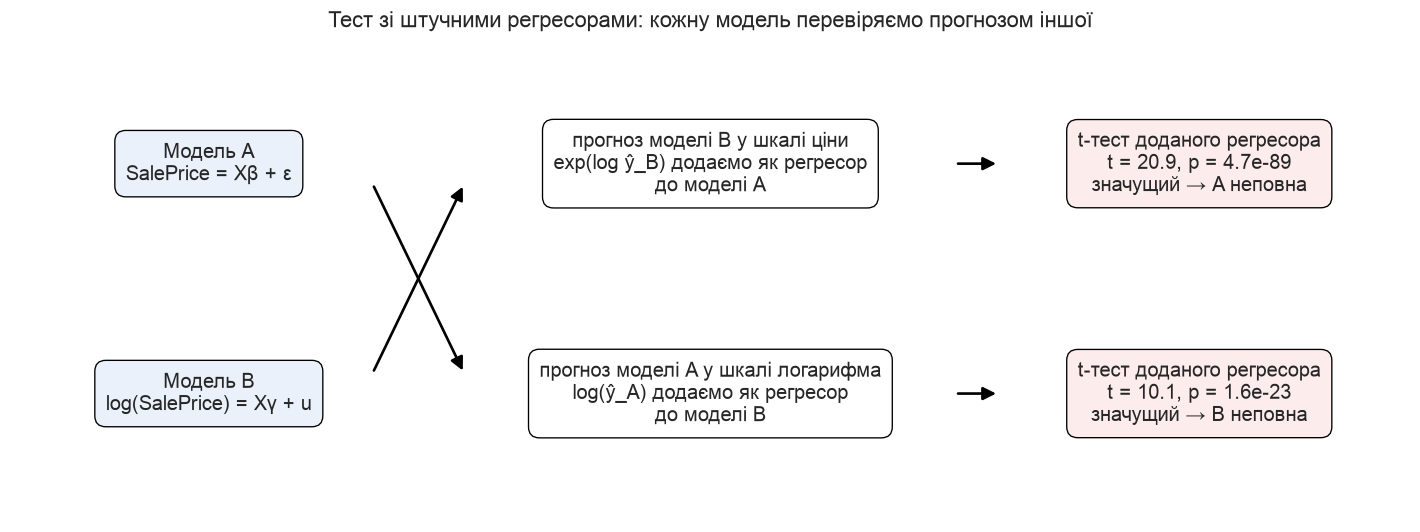
\includegraphics[width=\linewidth,height=0.82\textheight,keepaspectratio]{../../figures/problem5_jtest.png}
\caption{Схема тесту зі штучними регресорами: прогноз кожної моделі переводимо в шкалу іншої.}
\end{figure}


\begingroup\fontsize{7.5}{9.5}\selectfont\setlength{\tabcolsep}{2.5mm}\renewcommand{\arraystretch}{1.15}
\par\vspace{2pt}\noindent\begin{tabular}{|lllll|}
\hline
Нульова специфікація & t звичайний & p звичайне & t HC1 & p HC1 \\
\hline
SalePrice \textasciitilde{} X & 20.9046 & 4.68683e-89 & 6.42438 & 1.60109e-10 \\
log(SalePrice) \textasciitilde{} X & 10.1076 & 1.55684e-23 & 5.17715 & 2.44653e-07 \\
\hline
\end{tabular}\par\vspace{2pt}
\endgroup


\begingroup\fontsize{7.5}{9.5}\selectfont\setlength{\tabcolsep}{2.5mm}\renewcommand{\arraystretch}{1.15}
\par\vspace{2pt}\noindent\begin{tabular}{|llll|}
\hline
 & AIC зі statsmodels & AIC для щільності y & BIC для щільності y \\
\hline
SalePrice & 55370.7 & 55370.7 & 55897.5 \\
log(SalePrice) & -3214.31 & 54756.8 & 55283.6 \\
\hline
\end{tabular}\par\vspace{2pt}
\endgroup


\answerheading
Порівнюємо дві моделі з тими самими 28 відібраними змінними:
\[(A)\ y=X\beta+\varepsilon,\qquad (B)\ \log y=X\gamma+u,\qquad y=SalePrice.\]
де \(X\) позначає матрицю відібраних регресорів із константою, \(\beta\)
і \(\gamma\) вектори коефіцієнтів, \(\varepsilon\) і \(u\) похибки.

Тест зі штучними регресорами виконуємо в обох напрямках (схема на
рисунку вище):

\begin{enumerate}
\def\labelenumi{\arabic{enumi}.}
\item
  До моделі \(y\) додаємо прогнози лог-моделі, переведені у шкалу ціни:
  \(\exp(\widehat{\log y})\).
\item
  До моделі \(\log y\) додаємо логарифм прогнозів моделі ціни:
  \(\log(\widehat y)\). Перед цим перевіряємо, що всі \(\widehat y>0\).
\item
  В обох допоміжних регресіях перевіряємо \(H_0\): коефіцієнт доданого
  регресора дорівнює нулю. Якщо він значущий, поточна специфікація не
  врахувала інформацію, яку дає альтернативна.
\end{enumerate}

Ділення доданого регресора на 1000 у першій регресії змінює лише масштаб
його коефіцієнта, а не t-статистику. Експонента прогнозу логарифма сама
по собі не є оцінкою середньої ціни без додаткових припущень; тут це
допоміжний регресор для перевірки специфікації.

Код показує звичайні t-тести й додатково тести зі стандартними похибками
HC1, стійкими до гетероскедастичності. HC1 змінює стандартні похибки, а
не оцінки коефіцієнтів; висновок залишається наближеним.

Обидві специфікації відхиляються на рівні 0.05, зокрема й з HC1. Тест не
дає однозначного переможця: відхилення моделі A ще не доводить
правильності B. Це один із можливих результатів такого порівняння. Дані
вказують, що обидві прості форми залишають невраховані закономірності.

Чому не можна порівнювати AIC/BIC зі statsmodels напряму. Вони
стосуються різних залежних змінних і різних щільностей. Для лог-моделі
треба перейти від щільності \(\log y\) до щільності \(y\):
\[f_Y(y)=f_{\log Y}(\log y)/y,\qquad \ell_B^{(y)}=\ell_B-\sum_i\log y_i.\]
де \(f_Y\) і \(f_{\log Y}\) позначають щільності ціни та її логарифма,
\(\ell_B\) логарифм правдоподібності моделі B для \(\log y\),
\(\ell_B^{(y)}\) її логарифм правдоподібності у шкалі \(y\).

Тому до AIC та BIC лог-моделі додаємо \(2\sum_i\log y_i\).

Після поправки обидва критерії віддають перевагу лог-моделі серед цих
двох кандидатів. Але це не скасовує результат тестів: жодну з них не
можна вважати підтвердженою правильною специфікацією. Менший AIC також
не гарантує меншої MSE прогнозу ціни в доларах.

RSS мають різні одиниці, а \(R^2\) безрозмірний, проте описує варіацію
різних відгуків. Тому їхнє пряме порівняння для \(y\) і \(\log y\)
некоректне. Через важкі хвости, впливові точки та попередній відбір
змінних наведені p-значення слід сприймати як наближену діагностику.


\Needspace{212.0pt}

\subsection{(11) Крос-валідація}

\begin{taskstatement}
Ми хочемо оцінити прогнозну здатність побудованої регресії. Розглянемо
повну модель та модель після відбору ознак. Порівняйте ці дві моделі за
допомогою крос-валідації «залишення по одному» (LeaveOneOut) та
5-блочної крос-валідації (KFold) з бібліотеки sklearn.model\_selection.
Поясніть ідею цієї техніки за допомогою формул та зробіть висновок про
прогностичну здатність обох моделей на основі метрики MSE.
\end{taskstatement}


\pythoncode{p5-c35}

\begingroup\fontsize{7.5}{9.5}\selectfont\setlength{\tabcolsep}{1.5mm}\renewcommand{\arraystretch}{1.15}
\par\vspace{2pt}\noindent\begin{tabular}{|>{\raggedright\arraybackslash}p{25.15mm}>{\raggedright\arraybackslash}p{22.43mm}>{\raggedright\arraybackslash}p{19.42mm}>{\raggedright\arraybackslash}p{28.43mm}>{\raggedright\arraybackslash}p{32.14mm}>{\raggedright\arraybackslash}p{19.42mm}|}
\hline
Схема & Модель & Параметрів & MSE навчальне, дол.² & MSE крос-валідації, дол.² & RMSE, дол. \\
\hline
LeaveOneOut & Повна & 269 & 4.18001e+08 & 9.55734e+08 & 30915 \\
LeaveOneOut & Після відбору & 91 & 4.96967e+08 & 9.15862e+08 & 30263.2 \\
KFold (5 блоків) & Повна & 269 & 4.18001e+08 & 9.55302e+08 & 30908 \\
KFold (5 блоків) & Після відбору & 91 & 4.96967e+08 & 9.13883e+08 & 30230.5 \\
\hline
\end{tabular}\par\vspace{2pt}
\endgroup


\begingroup\fontsize{7.5}{9.5}\selectfont\setlength{\tabcolsep}{2.5mm}\renewcommand{\arraystretch}{1.15}
\par\vspace{2pt}\noindent\begin{tabular}{|lll|}
\hline
Повна & Після відбору & Order \\
\hline
-660415 & -650715 & 1499 \\
-549931 & -540751 & 2181 \\
-439550 & -431852 & 2182 \\
199807 & 195993 & 514 \\
154980 & 168660 & 1761 \\
\hline
\end{tabular}\par\vspace{2pt}
\endgroup


\Needspace{28.4pt}

\resulttext{p5-c35-out2.txt}

\begin{figure}[H]
\centering
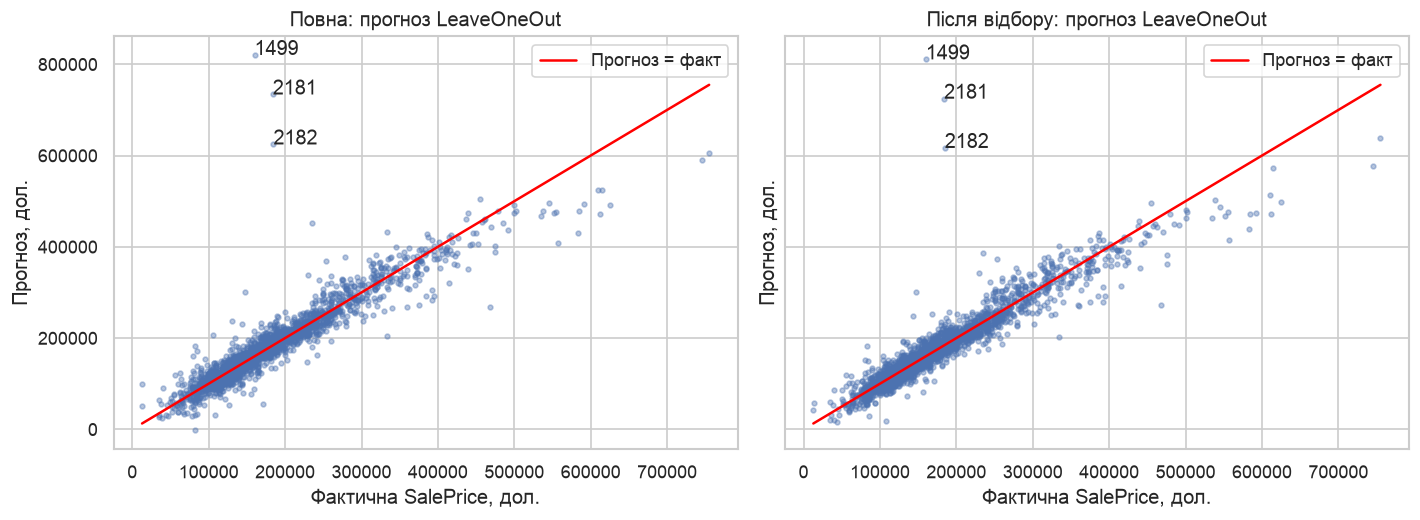
\includegraphics[width=\linewidth,height=0.82\textheight,keepaspectratio]{../../figures/problem5_cv.png}
\caption{Фактичні ціни та прогнози LeaveOneOut для двох моделей.}
\end{figure}


\answerheading
Ідея крос-валідації: кожен прогноз отримуємо з моделі, яку навчали без
відповідного тестового рядка. Навчальна MSE зазвичай оптимістична, бо
коефіцієнти вже підігнано до цих цін.

LeaveOneOut: для кожного \(i\) навчаємо модель на \(n-1\) рядках і
прогнозуємо пропущений:
\[MSE_{LOO}=\frac1n\sum_{i=1}^n(y_i-\widehat y_i^{(-i)})^2.\] де
\(\widehat y_i^{(-i)}\) позначає прогноз для рядка \(i\) з моделі,
навчаної без нього, \(n=2414\). Це 2414 підгонок для кожної моделі.

KFold: ділимо рядки на 5 блоків \(V_1,\ldots,V_5\)
(\texttt{shuffle=True}, \texttt{SEED=42}). Кожен блок один раз є
тестовим, інші чотири навчальними:
\[MSE_5=\frac1n\sum_{v=1}^5\sum_{i\in V_v}(y_i-\widehat y_i^{(-V_v)})^2.\]
де \(\widehat y_i^{(-V_v)}\) позначає прогноз із моделі, навчаної без
блоку \(V_v\), до якого належить рядок \(i\). Це 5 підгонок для кожної
моделі. Обидві моделі використовують ті самі розбиття.

Порівнюємо повну та відібрану моделі ціни в доларах, як вимагає пункт
11. У пункті 10 лог-модель мала кращі інформаційні критерії, але обидві
специфікації були відхилені; її прогнозну MSE тут не оцінюємо.
\texttt{LinearRegression} і OLS дають однакові підгонки для тієї самої
матриці регресорів.

Висновок:

\begin{itemize}
\item
  На навчальних даних повна модель має меншу MSE. Для вкладених моделей
  на тих самих рядках додавання регресорів не може збільшити мінімальний
  RSS.
\item
  У цих розбиттях відібрана модель має меншу MSE: приблизно на 4.2\% для
  LOO і на 4.3\% для KFold. Вона простіша й тут прогнозує трохи точніше;
  це узгоджується з ризиком перенавчання повної моделі, але не доводить,
  що всі додаткові параметри підганяли лише шум.
\item
  LOO та KFold дали близькі оцінки. Для відібраної моделі RMSE становить
  приблизно 30.3 тис. дол.; це корінь із середнього квадрата помилки, а
  не гарантія такої похибки для кожного будинку.
\item
  Великий внесок у MSE дають Order 1499, 2181 і 2182: помилки відібраної
  моделі приблизно 651, 541 і 432 тис. дол. Без їхніх помилок MSE LOO
  була б \(5.705\cdot10^8\) та \(5.427\cdot10^8\) для повної й
  відібраної моделей. Це лише аналіз внеску точок у метрику; у головному
  результаті всі продажі залишено.
\item
  Якщо індикатор категорії дорівнює 1 лише для тестового будинку, у
  навчальній частині весь його стовпець нульовий.
  \texttt{LinearRegression} задає такому коефіцієнту 0: модель не може
  навчитися ефекту відсутнього рівня. Це пояснює великі помилки для
  Order 1499 і 2181.
\end{itemize}

Обмеження: набір змінних обрано за BIC на всіх 2414 рядках. Тому це
порівняння двох зафіксованих специфікацій, а не незалежна оцінка всього
алгоритму відбору. Для останньої відбір треба повторювати всередині
кожної навчальної частини; поточна оцінка відібраної моделі може бути
оптимістичною. Різниця близько 4\% сама по собі не доводить статистичної
переваги на інших вибірках.

